\chapter{Experiments \& Evaluations}
\label{chapter:evaluation}

\section{Overview}
In this chapter, we start with exploring how we evaluate the experiments and what metrics we use to measure them in Section \ref{section:eval}. Next, in Section \ref{section:trit} we discuss the experimental setup and the system used for the experiments. To better understand the impact of data in ASR experiments, we run multiple training configurations using different amounts of data in Section \ref{section:res_scale}. Then, in Section \ref{section:res_dist} we analyse the impact of distributed training and evaluate the impact of using multi \acrshort{gpu}, multiprocess techniques on training time and \acrshort{wer}. Next, we try to match hyperparameters of distributed training exactly with normal training to check the direct time comparisons of convergence time. In Section \ref{section:20000wer}, we compare the runs for 20,000 hours dataset with different methods of training. Next, we analyse the effect of accent of the \acrshort{wer} in Section \ref{section:accentwer}. Finally, we evaluate our model with other publicly available datasets and report the \acrshort{wer}s on those test sets.


\section{Experimental Setup}
\label{section:trit}
For all of our experiments, we use Aalto University's Triton\footnote{Triton cluster, Aalto scientific computing \href{https://scicomp.aalto.fi/triton/}{https://scicomp.aalto.fi/triton/}}, a high-performance computing cluster. Triton has an Nvidia DGX-1\footnote{Nvidia DGX, Wikipedia \href{https://en.wikipedia.org/wiki/Nvidia_DGX}{https://en.wikipedia.org/wiki/Nvidia\_DGX}} machine which contain 8 Tesla V100 \acrshort{gpu}s and are optimized for deep learning applications. Each GPU has a 32 GB memory with CUDA compute 7.0 capability. These \acrshort{gpu}s are used for all the deep learning training jobs, including the multi-\acrshort{gpu} ones. This research work also required large amounts of storage that can be accessed from multi processes and from multiple nodes at the same time, we use the Lustre\footnote{Lustre \href{https://www.lustre.org/}{https://www.lustre.org/}} filesystem which is a scalable filesystem which provides large storage capacity and high sequential throughput for cluster-based applications. The lustre storage is connected via an Infiniband\footnote{InfiniBand, Wikipedia. \href{https://en.wikipedia.org/wiki/InfiniBand}{https://en.wikipedia.org/wiki/InfiniBand}} connection, which features high throughput and low latency.

\section{Evaluation Criteria}
\label{section:eval}
We monitor the training jobs using TensorBoard. The main metrics that we track are training loss value, validation loss and validation \acrshort{wer}. The input transcript follows the typical conventions for capitalization and punctuation, as discussed in Section \ref{section:bizspeech}. In the initial stages of experiments, we did not take steps to remove punctuation marks and capitalization from the input text, and this led to the acoustic model being trained end to end along with the capitalization and punctuation marks in them. Hence, for the later experiments, we stuck with this setup because we noticed that the model was able to predict the capitalization and punctuation marks in many cases. During post-processing, we apply text normalization and report word error rates, based on the test split of the dataset, with and without punctuations or capitalization. Therefore, for all experiments we have a \acrshort{wer} with punctuations considered and without punctuations in them. We also report the \acrlong{cer} with punctuations for the test set. Table \ref{table:splits} show the train, validation, and test data splits details.

\begin{table}[ht]
\centering
\begin{tabular}{ c | c  c }
\hline
  & Utterances & Hours \\
 \hline
 \verb|Train| & 8809282 & 20000 \\ 
 %\hline
 \verb|Validation| & 186165 & 413 \\ 
 %\hline
 \verb|Test| & 185623 & 412 \\ 
 \hline
\end{tabular}
\caption{\label{table:splits}Dataset Train Validation Test Statistics }
\end{table}

\section{Experiments overview}
\label{section:exp_desc}
We use \inlinecode{SentencePiece} Tokenizer with vocabulary size of 5k with \emph{bpe} as the token type. The detokenized output from the acoustic model consists of upper case characters, lower case characters, digits, punctuation marks, percent sign, currency notations, space character, a token for filler words ("--"), hence covering all the characters present in the dataset transcriptions. The model used is an attention-based encoder decoder model. For the encoder, we use a \acrshort{crdnn} model. The convolution part of the \acrshort{crdnn} model has 2  blocks. Each block has 2 convolution layers with \inlinecode{LayerNorm} applied and \inlinecode{LeakyReLU} activation function. These two convolution layers are then followed by \inlinecode{MaxPool} and \inlinecode{Dropout} layers. The two major blocks are chained together, and then the output is passed to a bidirectional-\acrshort{lstm} cell with 512 neurons. The output of the recurrent part of the neural network is passed to the \acrshort{mlp} portion of the network. This has two blocks of Linear Layer with \inlinecode{BatchNorm} and \inlinecode{LeakyReLU} activation function with \inlinecode{Dropout}. We then use the output of the encoder is fed to the decoder part of the network. The decoder is a location aware attentional \acrshort{rnn} with a \acrshort{gru} cell with the attention dimension set to 512. Appendix \ref{chapter:model-architecture} shows the complete model architecture and complete hyperparameter configuration in sown in \ref{chapter:hyparam}. We use Adam optimizer with learning rate set to 0.0001 without any scheduler. We apply \acrshort{ctc} loss for the initial 15 epochs and then disabled it for further training. The final model is the checkpoint with the best validation word error rate. The target batch size used was 180 seconds, with a maximum batch size of 240 seconds. The batch size is represented in seconds because of the dynamic batching method explained in Section \ref{section:dynbatch}. We do not use external language models to evaluate the final metrics.  

\section{Dataset size-based experiments}
\label{section:res_scale}
We performed experiments to compare the models between the different scales of data used for training jobs. We run training jobs using 80, 200, 2000, 8000 and 20000 hours. For all the data scales, we spawn two processes for data loading and preprocessing. The different dataset splits that were used are shown in Table \ref{table:datascales}. All the experiments are run using the same hyperparameters. 

\begin{table}[ht]
\centering
\begin{tabular}{c c c c c c}
\hline
  Hours & Utterances & WER & WER-P & CER-P & Time to Benchmark\\
 \hline
  80 & 38246 & 46.73\% & 50.38\% & 29.63\% & 42\textsuperscript{*}\\ 
  200 & 94840 & 43.84\% & 47.84\% & 29.08\% & 64\textsuperscript{*}\\
  2000 & 964824 & 33.76\% & 38.52\% & 27.8\% & 140\textsuperscript{*}\\
  8000 & 3480514 & 20.74\% & 24.31\% & 12.04\% & 76\\
  20000 & 8809282 & 14.01\% & 17.12\% & 7.67\% & 48\\
 \hline
\end{tabular}
\caption{\label{table:datascales}Dataset Split for training at different scales. Hours column shows the number of training data used for the experiments. The utterances column shows the number of training utterances for each data split. WER is word error rate without punctuations, WER-P is the word error rate considering the punctuations and capitalizations, CER-P is the character error rate with the punctuations and capitalizations. Time to convergence is the wall clock time taken for the training to reach the benchmark WER. \textsuperscript{*} indicates that the training never reached the benchmark accuracy, and the hours are the total hours training was run.}
\end{table}

Note that for evaluation, we use the same test and validation sets across all the scales to make it convenient to compare the results. Since we create the test and validation splits with the largest dataset (20000 hours) in mind, they are larger than the training sets for 80 and 200 hour datasets. Predictably, the word error rates drop with the increase in the scale of training data, and we see a similar trend with the character error rates. The difference between the word error rates with and without text normalization is at an almost constant 3.5\% points. The CER-P is also an important metric for our dataset because of the presence of punctuation and capitalization in the transcript. We also report training time to convergence. This is measured by having a benchmark \acrshort{wer} of 19.74\%, which is the Azure's WER on random utterances from the dataset, discussed in Section \ref{section:bizspeech}. So, \emph{time to convergence here is defined as the training wall clock time for the model to reach the validation word error rate of 19.74\%}. We see that the larger dataset reached the benchmark \acrshort{wer} before the smaller 8000 hour dataset. We hypothesize that the more diverse dataset helped to generalize better, and this led to quicker and better convergence of the model. This further showcases the importance of large-scale training tasks, even when training time is an important factor taken into consideration.

\section{Distributed Training}
\label{section:res_dist}
All the experiments discussed above are run using a single GPU and a single process. This section now delves into the distributed training experiments. 

\subsection{Synchronous training}
We use the \acrfull{ddp} approach, which is a Data parallel, synchronous training method which uses the \inlinecode{allreduce} operation to keep the weights synchronized. In these experiments, we spawn 4 processes, each with access to a discrete GPU. The same model is copied to all the \acrshort{gpu}s. Each process computes the forward pass and the loss and gradients to backpropogate, and for each GPU, we also spawn two processes for data loading and preprocessing on the fly. For using multiple \acrshort{gpu}s, the batch size becomes a vital hyperparameter. If we retain the same batch size as that was used for the single \acrshort{gpu}, the overall effective batch size is the number of GPUs used times the single batch size. Table \ref{table:wer_ddp} shows the word error rates for these experiments. For the \acrshort{ddp} experiments, we use 4 GPUs, with the effective batch size hence becomes 4 times the individual batch size. 

\begin{table}[ht]
\centering
\begin{tabular}{c | c c c | c c c }
\hline
\textbf{Train Data} & \multicolumn{3}{c|}{\textbf{8000}} & \multicolumn{3}{c}{\textbf{20000}}\\\cline{2-7}
   \textbf{Size (in hrs)} & WER & WER-P & CER-P & WER & WER-P & CER-P\\
 \hline
  Single GPU & 20.74\% & 24.31\% & 12.04\% & 14.01\% & 17.12\% & 7.67\%\\
  4-GPU DDP & 17.38\% & 20.65\% & 10.16\% & 10.87\% & 13.69\% & 5.73\% \\
 \hline
\end{tabular}
\caption{\label{table:wer_ddp} WER, WER-P and CER-P comparison for single GPU and multi GPU runs.}
\end{table}

We compare the distributed data parallel results with the single GPU results. We observe improvement of 15\%-38\% in \acrshort{wer}. This can be attributed to the fact that larger batch sizes work better for the hyperparameter configuration and model architecture setup because everything apart from that is kept constant. Hence, the use of DDP is perfect for these experiments since it enables usage of larger batch sizes. From these experiments, it is apparent that using DDP is beneficial, especially in cases where larger batch sizes lead to better convergence of the models. 


\begin{table}[ht]
\centering
\begin{tabular}{c | c c c | c }
\hline
     & WER & WER-P & CER-P & Time to Benchmark\\
 \hline
  1-GPU & 20.74\% & 24.31\% & 12.04\% & \textbf{59} \\
  1-GPU \acrshort{sga} & 16.74\% & 19.98\% & 7.60\% & \textbf{80} \\
  4-GPU DDP & 17.38\% & 20.65\% & 7.67\% & \textbf{42} \\
 \hline
\end{tabular}
\caption{\label{table:wer_ddp_grad} WER, WER-P and CER-P comparison for single GPU, single GPU with sequential gradient accumulation and multi GPU runs for the 8000 training hours dataset. The table also shows the wall clock time to convergence with the different setups.}
\end{table}

Hence, to make comparisons on the time to convergence of the models, we try to level the batch sizes for the two setups. One way would be to reduce the batch size by a factor of the number of GPUs used for the DDP setup. However, this means that the efficiency of the training takes a hit. Therefore, we choose a different method to achieve consistency between the setups. Since the gradients in the multiple GPU setup are updated 4 batches at a time by computing them in parallel, we apply the backward pass after accumulating the gradients for 4 batches, processed sequentially using a single \acrshort{gpu}. This effectively means that the batch size is increased by a factor of 4. We call this method \acrfull{sga}. In this method, we compute the forward pass, the loss, and the gradients for four batches sequentially and then run the backward passes together after processing the four batches. This makes the comparison more fair and easier to make. We conduct this experiment for the 8000 training hour dataset to get the results faster. We expect similar results with the larger dataset as well. 

\begin{figure}[ht]
  \begin{center}
    % below the size of the figure has been reduced for example
    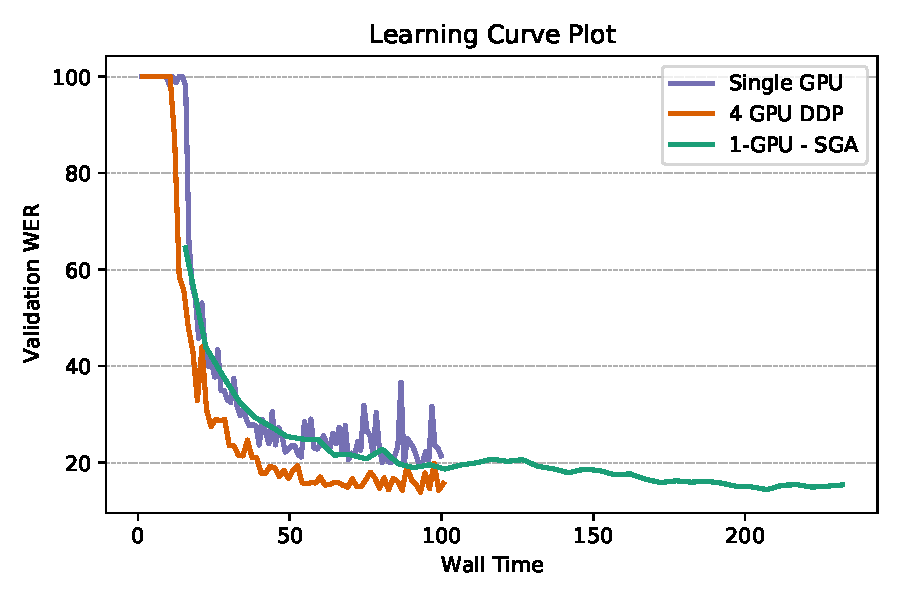
\includegraphics[width=\textwidth]{images/learning_curve_8000.pdf} 
    \caption{Learning curves during training for the different setups, with Validation WER on the y-axis and wall clock time in hours on the x-axis.}
    \label{fig:learningcurve_ddp}
  \end{center}
\end{figure}

We compare the word error rate for the \acrshort{sga} experiment with the other results in the Table \ref{table:wer_ddp_grad}. We see that the word error rates differ by around 0.5\% points between the \acrshort{sga} and the \acrshort{ddp} methods, and this can be attributed to minute variations like initial seeds and other random occurrences. We also report the time to convergence in the same table. We see that the single GPU run reached the benchmark \acrshort{wer} at around the 60 hours mark, which is 1.5 times the time to convergence of the 4-GPU DDP, but the single GPU model doesn't converge overall as much as the DDP run. Comparing the 1-GPU \acrshort{sga} and the 4-GPU \acrshort{ddp}, the time to convergence is half. The single GPU SGA takes 80 hours to reach the benchmark WER. Figure \ref{fig:learningcurve_ddp} shows the learning curve for the three runs, with the validation word error rate on the y-axis and wall clock time in hours on the x-axis. Note that we stop the training when the training loss was stagnant over at least 5 epochs. Again we see that the DDP plot reaches the benchmark \acrshort{wer} the quickest and converges sharply in the initial hours. 

\subsection{Asynchronous training}
Hogwild \cite{Niu2011HOGWILD:Descent} is used to evaluate the usage of asynchronous training. In this experiment, we store the weights on one single GPU, and we spawned 3 different processes to process the forward pass over different batches of data and calculate the loss and gradients to backpropogate. Then each process continues to update the weights on the GPU. Next, all individual processes again read the updated weights and continues to iterate over the next batches of data. We use 2 processes for each main process for data loading and preprocessing. Overall, the system works without any interlocking mechanism to ensure that the updates to the model weights are actually read by the other processes before being overwritten. Again, the batch size is a crucial hyperparameter because all the 3 processes use the same GPU, the same batch size as single process cannot be used as we will face issues managing the GPU memory. If we reduce the batch size for the single process experiment, the device efficiency reduces. Table \ref{table:wer_hog} shows the word error rates for these experiments. For the Hogwild experiments, we use 3 processes, and since each process acts on the same GPU, the batch size should be divided by the number of processes to keep the memory consumption about the same level, and thus the effective batch size is 1/3rd of the single GPU batch size.

\begin{table}[ht]
\centering
\begin{tabular}{c | c c c | c c c }
\hline
\textbf{Train Data} & \multicolumn{3}{c|}{\textbf{8000}} & \multicolumn{3}{c}{\textbf{20000}}\\\cline{2-7}
   \textbf{Size (in hrs)} & WER & WER-P & CER-P & WER & WER-P & CER-P\\
 \hline
  1-Process & 20.74\% & 24.31\% & 12.04\% & 17.38\% & 20.65\% & 10.16\%\\
  Hogwild & 22.4\% & 25.7\% & 12.70\% & 24.09\% & 27.56\% & 13.81\% \\
 \hline
\end{tabular}
\caption{\label{table:wer_hog} WER, WER-P and CER-P comparison for single process and 3 process distributed Hogwild runs for two data scales}
\end{table}

We compare the Hogwild results with the single GPU results. We observe a deterioration of 8\%-38\% in \acrshort{wer} with using Hogwild. This can be attributed to the fact that smaller batch sizes work does not work well for the hyperparameter configuration and model architecture setup because all the other configurations is the same. Hogwild also doesn't improve by adding more data. We see that the accuracy metrics are better for the 8000 hours training set. Similar to the synchronous training experiments, comparing these results which have different effective batch sizes is not reasonable. 

\begin{table}[ht]
\centering
\begin{tabular}{c | c c c | c }
\hline
     & WER & WER-P & CER-P & Time to Benchmark\\
 \hline
  1-Process & 20.74\% & 24.31\% & 12.04\% & \textbf{35} \\
  1-Process $\frac{1}{3}$ BS & 24.16\% & 27.75\% & 14.91\% & \textbf{54} \\
  3-Process Hogwild & 22.4\% & 25.7\% & 12.70\% & \textbf{46} \\
 \hline
\end{tabular}
\caption{\label{table:wer_hog_seq} WER, WER-P and CER-P comparison for single GPU, single process with one third batch size and multi GPU runs for the 8000 training hours dataset. The table also shows the wall clock time to convergence with the different setups.}
\end{table}

Hence, to make the comparisons on the time to convergence of the models, we use sequential updates to simulate multiple process settings on a single process system. We reduce the batch size of the single process experiment to one third the size of the regular batch size, and this equates it to the Hogwild experiment closely. This makes the comparison more fair and easier to make. We conduct this experiment for the 8000 training hour dataset to get the results faster.  We expect similar results with the larger dataset as well. Since Hogwild never reaches \acrshort{wer} of 19.74\%, we use a word error rate of 30\% as the benchmark to compare the time of convergence. Table \ref{table:wer_hog_seq} shows the word error rate for the single process with reduced batch size, compared to the other results, along with  wall time to convergence (at 30\% WER) in hours. We see that Hogwild does slightly better in word error rates and character error rates than the sequential update with reduced batch size. Comparing the time to convergence, we see that the single process run converges quickest, but along the experiments which uses the same effective batch size, Hogwild converges around 8 hrs quicker than the sequential update simulation of Hogwild. 

\begin{figure}[ht]
  \begin{center}
    % below the size of the figure has been reduced for example
    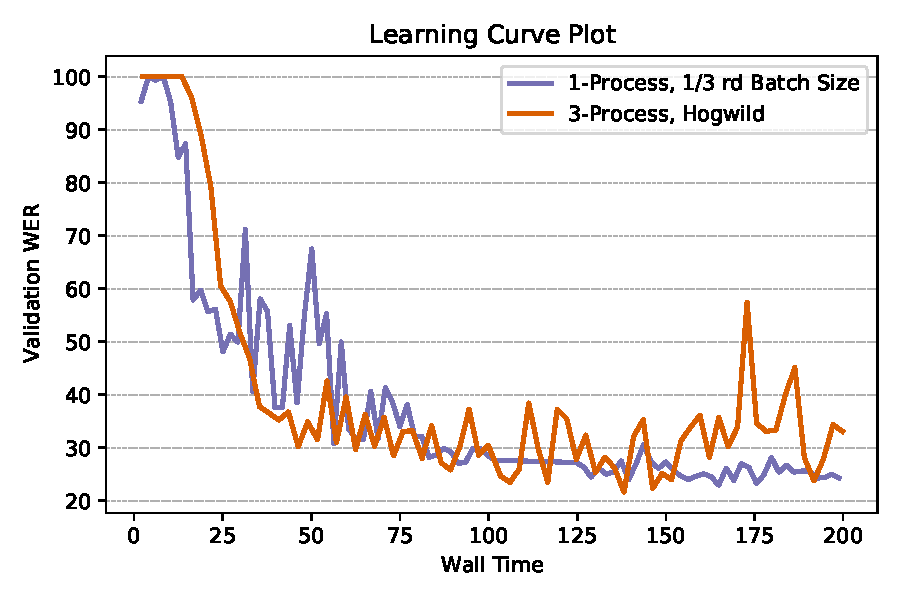
\includegraphics[width=\textwidth]{images/learning_curve_8000_hogwild.pdf} 
    \caption{Learning curves during training for the different setups, with Validation WER on the y-axis and wall clock time in hours on the x-axis.}
    \label{fig:learningcurve_async}
  \end{center}
\end{figure}

Figure \ref{fig:learningcurve_async} shows the learning curve for the two runs, with the validation word error rate on the y-axis and wall clock time in hours on the x-axis. We stop the training, when the training loss is stagnant over at least 5 epochs. The learning curves are quite erratic, and we observe a lot of variation in validation word error rates even when the training loss vales are constant. 


\section{Interpreting the WER results}
\label{section:20000wer}
Our experiments show the different methods to accelerate all the different parts of the pipeline for training ASR models for data scalability. We now report the word error rate, word error rate with punctuations and capitalizations considered and the character error rate among the three different methodologies. The first method is the centralized training with a single GPU with multiprocessing used only for data loading and preprocessing. The second methodology is the Distributed Data Parallel method, which is the synchronous training using 4 GPUs, with one process on each GPU for training. The third method is the asynchronous training with Hogwild, with 3 processes using a single GPU to share weights and update them in parallel. These results are reported in Table \ref{table:overall_wer}. but to compare the training methods for large-scale datasets and to showcase the best workflow for such experiments, we now compare the different metrics for the largest training dataset size, i.e. 20,000 hours. 
\begin{table}[ht]
\centering
\begin{tabular}{c | c c c | c }
\hline
     & WER & WER-P & CER-P & Training Wall-time (hrs)\\
 \hline
  1-GPU & 14.01\% & 17.12\% & 7.67\% & \textbf{59} \\
  4-GPU DDP & 10.87\% & 13.69\% & 5.73\% & \textbf{32} \\
  1-GPU Hogwild & 24.09\% & 27.56\% & 13.81\% & \textbf{100\textsuperscript{*}} \\
 \hline
\end{tabular}
\caption{\label{table:overall_wer} WER, WER-P and CER-P comparison for single GPU, single GPU, multi GPU \acrshort{ddp}, 1-GPU Hogwild runs for the 20,000 training hours dataset. The table also shows the wall clock time to convergence with the different setups. \textsuperscript{*} indicates that the training never reached the benchmark accuracy, and the hours are the total hours training was run.}
\end{table}

The synchronous \acrshort{ddp} training job with \acrshort{wer} of 10.87\% and \acrshort{cer}-P of 5.73\% is the best result obtained overall. Synchronous training methods work well when the different \acrshort{gpu}s are similar in their processing power and memory storage. This avoids stragglers and training synchronization can happen smoothly. This can also be seen in our experiments that the time to convergence is reduced by half with the use of \acrshort{ddp} on multiple GPUs. 

Some caution has to be taken before reading these results, because the hyperparameters were optimized only once at the beginning of the experiments, and it is possible that for the different methods, varying the hyperparameters could lead to better results. The main aim of this thesis was not to get the best \acrshort{wer} for the dataset but to evaluate the best practices and methods for data scalability, and hence this step was not given much prominence during the experiments. 

\section{Effect of accent on the WER}
\label{section:accentwer}
In Section \ref{section:bizspeech}, we had discussed the challenges in the dataset concerning the utterances which are spoken by people from different parts of the world, including non-native speakers of English, which is particularly interesting and useful for building a diverse model. We compare the word error rates for our best model with Google's Azure's results and also analyse the drop in accuracy between native and non-native utterances in Figure \ref{fig:wer_cloud_final} 

\begin{figure}[ht]
  \begin{center}
    % below the size of the figure has been reduced for example
    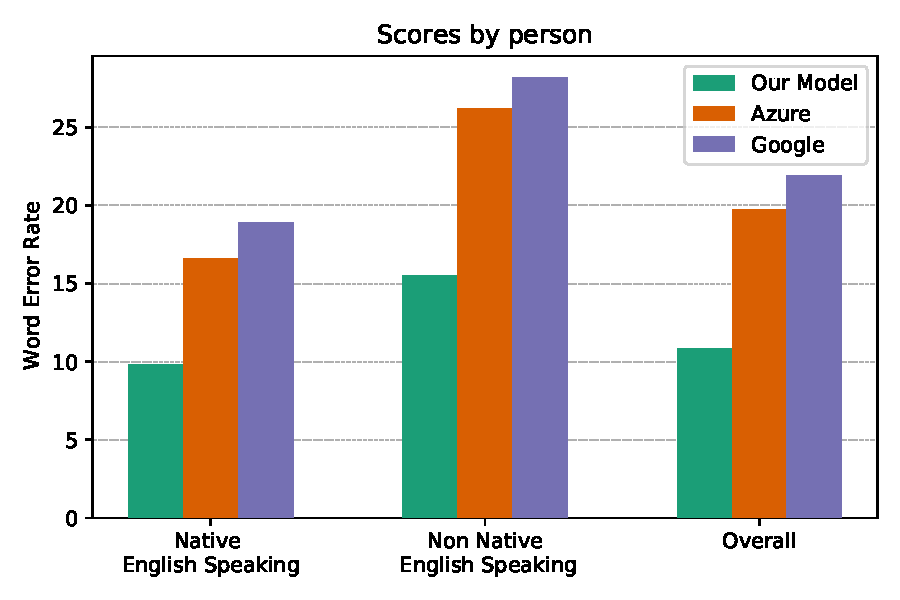
\includegraphics[width=\textwidth]{images/wer_cloud_final.pdf} 
    \caption{Word error rates comparison for native and non-native speakers of English between Google, Azure and our models.}
    \label{fig:wer_cloud_final}
  \end{center}
\end{figure}

The word error rates for the native and non-native speakers are calculated on different utterances for our model. This is due to overlap between the utterances used for cloud services to estimate \acrshort{wer} and the training set of our model. There is a consistent degradation of performance pertaining to non-native English speakers.


\section{Evaluation with other datasets}
Here we report the results with our models for other datasets and compare them to the metrics with our models. 
\subsection{SPGISpeech}
SPGISpeech \cite{Oneill2021SPGISpeech:Recognition}, as discussed in Section \ref{section:bizspeech} is quite similar to BizSpeech dataset, and we evaluate our best model on their dataset. The authors of SPGISpeech have reported their results on the \inlinecode{test} split of the dataset, but have made only the \inlinecode{val} and \inlinecode{train} splits public. Hence, we evaluate our model on the \inlinecode{val} split of the model. Table \ref{table:spgi} shows the \acrshort{wer} and \acrshort{wer}-P for the \inlinecode{val} split on our model sets along with the results from the Conformer \cite{Gulati2020Conformer:Recognition} \ model with \inlinecode{test} split results from SPGISpeech experiments.
\begin{table}[ht]
\centering
\begin{tabular}{c | c c  }
\hline
\textbf{Results} & WER & WER-P \\
 \hline
  Our Model & 8.66\% & 15.26\% \\
  SPGISpeech \cite{Oneill2021SPGISpeech:Recognition} & 2.3\% & 5.7\% \\
 \hline
\end{tabular}
\caption{\label{table:spgi} WER and WER-P comparison for val split of SPGISpeech using our best model and test split with the Conformer model from SPGISpeech experiments.}
\end{table}

The normalized \acrshort{wer} on SPGISpeech of 8.66\% is less than the best word error rate obtained on BizSpeech, which indicates that the data in the SPGISpeech is much easier, because of the removal of data with currencies in them etc. The normalized \acrshort{wer} from SPGISpeech is reported after not only removing the casing of the text and punctuations, but also reduce the vocabulary while post-processing the text output to report the \acrshort{wer} results.  It is also important to note that the results are not on the same data split, and this will definitely have an impact on the \acrshort{wer}s. Since, the test split that was used by the authors is not available, it is impossible  to solve this difference.

\subsection{LibriSpeech}
Since the dataset size is big, we wanted to evaluate the model's generalization capabilities on  a dataset which is not related to BizSpeech. We employ similar strategy as the researchers of the People's Speech Dataset \cite{Galvez2021TheUsage}. We evaluate our best model on the LibriSpeech\cite{Panayotov2015Librispeech:Books} test datasets without any transfer learning, so the LibriSpeech data is completely unseen data for the model. Table \ref{table:libri} shows the test word error rates for LibriSpeech datasets and compare it with the People's Speech Dataset results. People's speech dataset consists of 30000 hours of diverse speech ranging from audiobooks, news, movies, commentaries, court hearings, etc. This makes the People's dataset quite close to the BizSpeech dataset, because of its size and diverse nature. Since LibriSpeech data does not contain any punctuations and capitalization, we normalize the hypothesis text from our model before calculating the \acrshort{wer} metrics. 

\begin{table}[ht]
\centering
\begin{tabular}{c | c c | c c }
\hline
\textbf{Results} & \multicolumn{2}{c|}{\textbf{test-clean}} & \multicolumn{2}{c}{\textbf{test-other}}\\\cline{2-5}
    & WER & CER & WER & CER\\
 \hline
  Our Model & 22.46\% & 10.62\% & 37.93\% & 20.41\%\\
  People's Speech \cite{Galvez2021TheUsage} & 32.17\% & 18.86\% & 57.56\% & 41.2\% \\
 \hline
\end{tabular}
\caption{\label{table:libri} WER and CER comparison for test-clean and test-other datasets with the People's Speech model}
\end{table}

Although, the results with our model are worse than state-of-the-art models on LibriSpeech, we manage to outscore the people's speech models by 30\% on the test-clean dataset and by 35\% on the test-other dataset which shows the model can generalize pretty well.
 
